\documentclass[11pt,a4paper]{report}

% ================= PACKAGES =================
\usepackage[margin=2.5cm]{geometry}
\usepackage{graphicx}
\usepackage{xcolor}
\usepackage{titlesec}
\usepackage{fancyhdr}
\usepackage{booktabs}
\usepackage{array}
\usepackage{enumitem}
\usepackage{tcolorbox}
\usepackage{hyperref}
\usepackage{caption}
\usepackage{fontspec}
\usepackage{tocloft}
\usepackage{longtable}
\newcolumntype{L}[1]{>{\raggedright\arraybackslash}p{#1}}
\usepackage{tikz}
\usetikzlibrary{arrows.meta,positioning,fit,backgrounds}

\setmainfont{Latin Modern Sans}[Scale=1.0]
\setmonofont{Latin Modern Mono}[Scale=0.9]

% ================= COLORS =================
\definecolor{primary}{HTML}{3C3489}
\definecolor{primarydark}{HTML}{26215C}
\definecolor{accent}{HTML}{1D9E75}
\definecolor{warn}{HTML}{B75E09}
\definecolor{lightgray}{HTML}{F1EFE8}
\definecolor{warnbg}{HTML}{FBF0E2}
\definecolor{bodytext}{HTML}{2C2C2A}
\definecolor{boxline}{HTML}{9C97C7}

\color{bodytext}

% ================= SECTION STYLING =================
\titleformat{\chapter}[display]
  {\normalfont\Huge\bfseries\color{primary}}
  {\chaptertitlename\ \thechapter}{10pt}{\Huge}
\titlespacing*{\chapter}{0pt}{0pt}{30pt}

\titleformat{\section}
  {\normalfont\Large\bfseries\color{primarydark}}{\thesection}{1em}{}
\titleformat{\subsection}
  {\normalfont\large\bfseries\color{primary}}{\thesubsection}{1em}{}

% ================= HEADER / FOOTER =================
\pagestyle{fancy}
\fancyhf{}
\renewcommand{\headrulewidth}{0.4pt}
\fancyhead[L]{\small\textcolor{primarydark}{SmartSchool -- School Management ERP}}
\fancyhead[R]{\small\textcolor{primarydark}{Software Design Document}}
\fancyfoot[C]{\thepage}

% ================= BOXES =================
\newtcolorbox{infobox}[1][]{
  colback=lightgray, colframe=primary, boxrule=0.6pt, arc=2pt,
  left=8pt, right=8pt, top=6pt, bottom=6pt, #1
}
\newtcolorbox{futurebox}[1][]{
  colback=warnbg, colframe=warn, boxrule=0.6pt, arc=2pt,
  left=8pt, right=8pt, top=6pt, bottom=6pt, #1
}

% ================= HYPERREF =================
\hypersetup{
  colorlinks=true,
  linkcolor=primary,
  citecolor=primary,
  urlcolor=accent,
  pdftitle={SmartSchool SDD - SEN4121 Large System Environment},
  pdfauthor={Group 2 -- ICT University Yaounde}
}

\captionsetup{font=small,labelfont={bf,color=primary}}

\newcommand{\sysname}{SmartSchool}

% ---- TikZ styles used throughout the diagrams ----
\tikzset{
  comp/.style={draw=primary, thick, rounded corners=2pt, fill=lightgray,
               minimum width=2.6cm, minimum height=1.05cm, align=center,
               font=\small\bfseries, text=primarydark},
  gwcomp/.style={comp, fill=primary!12},
  store/.style={draw=accent, thick, rounded corners=2pt, fill=accent!12,
               minimum width=2.4cm, minimum height=1.05cm, align=center,
               font=\small\bfseries, text=primarydark},
  ext/.style={draw=warn, thick, dashed, rounded corners=2pt, fill=warnbg,
               minimum width=2.6cm, minimum height=1.0cm, align=center,
               font=\small, text=primarydark},
  actorbox/.style={draw=primarydark, thick, rounded corners=6pt, fill=white,
               minimum width=2.1cm, minimum height=0.9cm, align=center,
               font=\small\bfseries, text=primarydark},
  usecase/.style={draw=primary, thick, ellipse, fill=white,
               minimum width=3.2cm, minimum height=0.95cm, align=center,
               font=\small, text=bodytext, inner sep=2pt},
  flow/.style={-Latex, thick, primary},
  asyncflow/.style={-Latex, thick, accent, dashed},
  entity/.style={draw=primary, thick, rounded corners=1pt, fill=white,
               align=left, font=\scriptsize, text=bodytext, inner sep=4pt},
  entityhead/.style={font=\bfseries\small, text=primarydark},
  rel/.style={-Latex, thick, boxline},
}

\begin{document}

% ================= TITLE PAGE =================
\begin{titlepage}
\begin{center}
\vspace*{1.2cm}

{\color{primary}\rule{\linewidth}{2pt}}

\vspace{0.8cm}
{\Huge\bfseries\color{primary} Software Design Document}

\vspace{0.4cm}
{\LARGE\color{primarydark} \sysname{} --- Student Records, Fee Invoicing\\[2pt] \& Staff Payroll Management System}

\vspace{0.6cm}
{\color{primary}\rule{\linewidth}{2pt}}

\vspace{2cm}

{\Large Prepared for: \textbf{ICT University Ya\'ound\'e}}

\vspace{0.3cm}
{\large Course: \textbf{SEN4121 -- Large System Environment} \quad (Practical Examination, Summer 2026)}

\vspace{0.3cm}
{\large Examiner: Engr. Tanwi Nkiamboh}

\vspace{1.5cm}

\begin{tabular}{ll}
\textbf{Document version:} & 1.0 \\[4pt]
\textbf{Group number:} & Group 2 \\[4pt]
\textbf{Date:} & \today \\[4pt]
\textbf{Status:} & Living document -- updated through Week 4 \\
\end{tabular}

\vspace{1cm}

\begin{tabular}{@{}p{6cm}p{4.5cm}@{}}
\toprule
\textbf{Group Member} & \textbf{Matricule} \\
\midrule
Kwete Rayan & ICTU20241377 \\
Kamdeu Yamdjeuson Neil Marshall & ICTU20241386 \\
Younga Tchappi Dylane & ICTU2241836 \\
Fru Chi Ehud Neba & ICTU20241812 \\
\bottomrule
\end{tabular}

\vfill

{\small\color{bodytext} This document describes the architecture, use cases,
data model, and behavioural design of \sysname{}, a microservice-based
school ERP built for the SEN4121 practical examination series. It reflects
the system as actually implemented through Week 4 (environment/auth,
database, microservices/gateway, messaging/security/performance), and marks
Week 5/6 elements explicitly as planned.}

\end{center}
\end{titlepage}

\tableofcontents
\clearpage

% ================================================================
\chapter{Introduction}

\section{Purpose}
This Software Design Document (SDD) describes the design of \sysname{}, a
school ERP built as a set of independently deployable microservices behind
a single API Gateway. It captures the system's architecture, static
structure (data model), and dynamic behaviour, and is intended to guide
implementation, the weekly oral evaluations, and future maintenance.

\section{Scope}
\sysname{} is organised into three functional modules, mirroring the exam
brief's Academic / Finance / HR split:
\begin{itemize}[leftmargin=1.4em]
  \item \textbf{Academic} --- students, courses, enrollments, and grades.
  \item \textbf{Finance} --- invoices, generated automatically from enrollments.
  \item \textbf{HR / Payroll} --- staff records and payroll (data model complete; service layer planned for Week 5).
\end{itemize}
Cross-cutting concerns -- authentication, the API Gateway, asynchronous
messaging, and security -- are treated as their own architectural layer
rather than duplicated per module.

\section{Definitions and Abbreviations}
See the SRS (Section 1.3) for the full glossary; the same terms apply here.

\section{Document Overview}
Chapter~2 gives the system architecture (component diagram). Chapter~3
presents the use-case model (use case diagram). Chapter~4 presents the
static structure (ER diagram and UML class diagram). Chapter~5 presents
dynamic behaviour (three sequence diagrams, a state diagram, an activity
diagram, and an object diagram). Chapter~6 documents the API design.
Chapter~7 covers security. Chapter~8 covers performance and reliability.
Chapter~9 covers deployment. Chapter~10 lists planned work for Weeks 5--6.
All eight UML diagrams (every one except the ER diagram, which uses ER
notation rather than UML) are generated from PlantUML source files under
\texttt{documentation/figures/smartschool/}, so the diagram and the text
describing it can never silently drift apart -- regenerating a figure is a
one-line command, not a manual redraw.

\section{Notation Used in This Document}
Every diagram in this document uses standard UML notation, drawn at full
strength (activation bars, guard conditions, composition/aggregation,
\texttt{<<include>>}/\texttt{<<extend>>}, swimlanes) rather than a
simplified subset. Table~\ref{tab:notation} is a single reference point for
every symbol used, so each diagram's own section can focus on what it shows
about \sysname{} specifically, not on re-explaining UML itself.

\begin{longtable}{L{3.0cm} L{6.4cm} L{4.6cm}}
\caption{UML and ER notation used throughout this document.}
\label{tab:notation} \\
\toprule
\textbf{Symbol} & \textbf{Meaning} & \textbf{Appears in} \\
\midrule
\endhead
Stick-figure actor & A human role (primary) interacting with the system & Use case diagram \\
Actor icon outside the system box, to the right & A \emph{secondary} actor: a supporting, non-human system the use case depends on, never the initiator & Use case diagram \\
Oval & A use case: one discrete unit of system behaviour & Use case diagram \\
Dashed arrow, \texttt{<<include>>} & Base use case \emph{always} incorporates the target use case's behaviour (arrow points to the included one) & Use case diagram \\
Dashed arrow, \texttt{<<extend>>} & The \emph{source} use case optionally adds behaviour to the target base use case, under a condition (arrow points to the base) & Use case diagram \\
Box, 3 compartments & A class: name, attributes, operations & Class diagram \\
Italic name/operation & Abstract class or abstract operation -- cannot be instantiated / has no body & Class diagram \\
\texttt{<<interface>>} stereotype & A contract with operations but no attributes or implementation & Class diagram \\
Hollow triangle, solid line & Inheritance / generalization (``is-a'') & Class diagram \\
Hollow triangle, dashed line & Realization -- a class implements an interface & Class diagram \\
Filled diamond & Composition -- the part's lifecycle is bound to the whole & Class, object diagrams \\
Hollow diamond & Aggregation -- a weaker ``has-a''; the part can outlive or be reassigned from the whole & Class, object diagrams \\
Plain line + multiplicity & Association, with how many instances relate on each end & Class, object diagrams \\
Underlined \texttt{name : Class} & An object diagram node: one specific instance, not a type & Object diagram \\
Box with plug icon & A component: a replaceable, encapsulated unit of implementation & Component diagram \\
Circle (``lollipop'') & A provided interface -- what a component offers & Component diagram \\
Dashed arrow, open head & A required interface or a dependency -- what a component needs & Component diagram \\
Vertical dashed line & A lifeline: one participant's timeline, top to bottom & Sequence diagrams \\
Solid arrow, filled head & A synchronous call -- the caller waits for a reply & Sequence diagrams \\
Solid arrow, open head & An asynchronous message -- the sender does not wait & Sequence diagrams \\
Dashed arrow & A return / reply message & Sequence diagrams \\
Narrow rectangle on a lifeline & Activation bar: the participant is actively processing for that span & Sequence diagrams \\
\texttt{alt} / \texttt{else} frame & Alternative fragments -- mutually exclusive branches & Sequence diagrams \\
Rounded rectangle & An action (one step) & Activity diagram \\
Diamond & A decision (one incoming, multiple guarded outgoing) or merge (multiple incoming, one outgoing) & Activity diagram \\
Solid horizontal bar & Fork (splits into concurrent flows) or join (synchronizes them back) & Activity diagram \\
Vertical column with a header & A swimlane -- which participant owns each action beneath it & Activity diagram \\
Filled circle / bordered filled circle & Initial node / activity-final node & Activity diagram \\
Rounded rectangle (state diagram) & A state, optionally with \texttt{entry}/\texttt{exit}/\texttt{do} actions & State diagram \\
\texttt{event [guard] / effect} & On a transition: what triggers it, the condition that must hold, and the side effect it causes & State diagram \\
\bottomrule
\end{longtable}

\section{Group Contributions}
\begin{center}
\begin{tabular}{@{}p{5cm}p{9cm}@{}}
\toprule
\textbf{Group Member} & \textbf{Contribution} \\
\midrule
Kwete Rayan & \\[10pt]
Kamdeu Yamdjeuson Neil Marshall & \\[10pt]
Younga Tchappi Dylane & \\[10pt]
Fru Chi Ehud Neba & \\[10pt]
\bottomrule
\end{tabular}
\end{center}

% ================================================================
\chapter{System Architecture}

\section{Architectural Style}
\sysname{} follows a \textbf{microservice architecture behind an API
Gateway}: every external client (the React frontend, curl, Postman, the
examiner) talks only to the Gateway, which is the sole component with a
port published to the host. Backend services are reachable only from other
containers on the internal Docker network. This satisfies the Week 3 build
task directly and gives each module (Academic, Finance) an independent
deployment and scaling unit.

\begin{infobox}
\textbf{Design principle.} The Finance Service never receives a direct call
to create an invoice. It reacts to an \texttt{enrollment.created} event on
its own schedule, so the Academic Service's request path is never coupled
to Finance Service's availability or latency.
\end{infobox}

\section{Component Diagram}
Figure~\ref{fig:arch} is a standard UML component diagram (notation key in
Table~\ref{tab:notation}) rather than a generic box-and-arrow sketch:
\begin{itemize}[leftmargin=1.4em]
  \item \textbf{Package boundary} -- the five components that make up \sysname{} itself (\texttt{React Frontend}, \texttt{API Gateway}, \texttt{Auth Service}, \texttt{Academic Service}, \texttt{Finance Service}) are grouped inside one package, visually separating ``the system'' from the external \texttt{Browser} actor and the two infrastructure nodes (\texttt{MySQL}, \texttt{RabbitMQ}).
  \item \textbf{Provided interface (lollipop)} -- \texttt{Gateway API /api/v1/**} is the \emph{only} interface exposed outside the package; the Frontend depends on it with a dashed arrow (a \emph{required} interface / dependency), and nothing outside the package can reach \texttt{Auth Service}, \texttt{Academic Service}, or \texttt{Finance Service} directly -- there is deliberately no lollipop on any of them.
  \item \textbf{Dependency arrows (dashed, open arrowhead)} -- every ``requires'' relationship: the Gateway on all three backend services (\texttt{requireAuth, proxy}), each service on MySQL (\texttt{mysql2 pool}), and the asynchronous publish/deliver pair through RabbitMQ.
  \item \textbf{Database and queue nodes} -- \texttt{MySQL} and \texttt{RabbitMQ} use their dedicated UML node shapes rather than generic components, since they are infrastructure the components depend on, not components of \sysname{} itself.
\end{itemize}

\begin{figure}[h!]
\centering
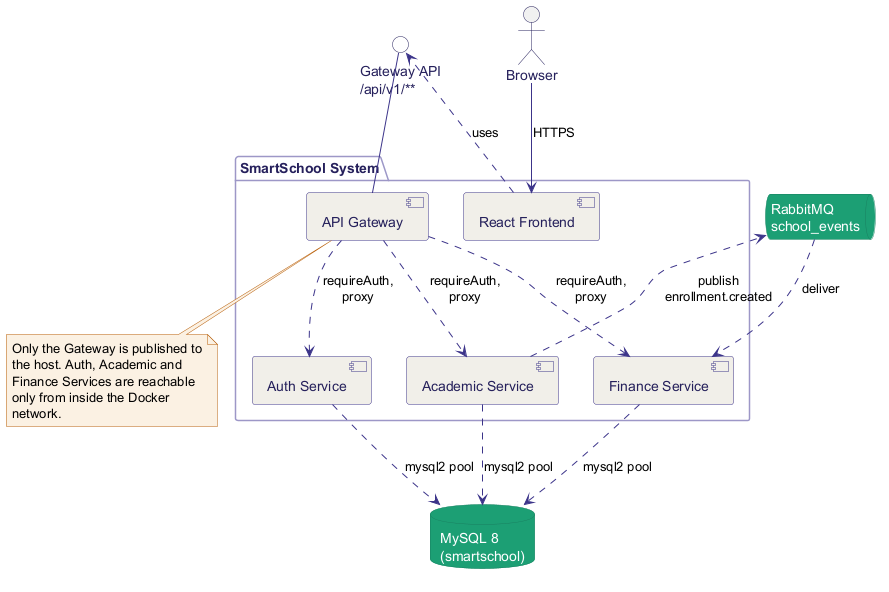
\includegraphics[width=0.95\linewidth]{figures/smartschool/09_component.png}
\caption{UML component diagram for \sysname{}: the Gateway is the only component with a provided interface reachable from outside the system package; every other dependency is internal (PlantUML source: \texttt{figures/smartschool/09\_component.puml})}
\label{fig:arch}
\end{figure}

\section{Component Responsibilities}
\begin{longtable}{L{3.0cm} L{11.0cm}}
\toprule
\textbf{Component} & \textbf{Responsibility} \\
\midrule
\endhead
API Gateway & Single public entry point. Verifies JWT signature/expiry on protected routes \emph{before} proxying (\texttt{requireAuth}); routes by URL prefix via \texttt{http-proxy-middleware}; rate-limits every route except \texttt{/health}; serves a combined Swagger UI at \texttt{/docs}. Does \emph{not} enforce role/ownership rules -- that is left to the owning service. \\
Auth Service & Owns the \texttt{users} table. Handles registration (bcrypt hashing), login (JWT issuance), \texttt{/me}, and a demo reporting endpoint gated to \texttt{admin}/\texttt{teacher}. \\
Academic Service & Owns \texttt{students}, \texttt{courses}, \texttt{enrollments}, \texttt{grades}. Enforces role/ownership rules per endpoint (e.g. a teacher may only grade their own courses). Publishes \texttt{enrollment.created} on successful enrollment. \\
Finance Service & Owns \texttt{invoices}. Serves \texttt{GET /api/invoices} and independently consumes \texttt{enrollment.created} to create invoices. \\
MySQL 8 & Single shared relational database (\texttt{smartschool}), one schema across all three modules, accessed by each service through its own connection pool with parameterized queries only. \\
RabbitMQ 3.13 & Message broker; one durable direct exchange (\texttt{school\_events}) and one durable queue (\texttt{invoice\_creation\_queue}) bound with routing key \texttt{enrollment.created}. Management UI on \texttt{:15672} for live inspection. \\
React Frontend & Single-page application (Vite + React). Holds the JWT and user profile in context, persisted to \texttt{localStorage}; calls the Gateway exclusively, never a backend service directly. \\
\bottomrule
\end{longtable}

% ================================================================
\chapter{Use Case Model}

\section{Actors}
\begin{center}
\begin{tabular}{@{}p{2.6cm}p{2.6cm}p{8.8cm}@{}}
\toprule
\textbf{Actor} & \textbf{Kind} & \textbf{Description} \\
\midrule
Admin & Primary & Creates courses, enrolls students on their behalf, views reports; highest privilege. \\
Teacher & Primary & Records grades for courses they teach; views reports alongside Admin. \\
Student & Primary & Registers, logs in, enrolls in courses, views their own enrollments, grades, and invoices. \\
Message Broker (RabbitMQ) & Secondary & Non-human, supporting actor: carries the \texttt{enrollment.created} event that drives asynchronous invoice creation. Never initiates a use case itself; supports one. \\
\bottomrule
\end{tabular}
\end{center}

\section{Use Case Diagram}
Figure~\ref{fig:usecase} shows the three primary (human) actors, the
secondary (system) actor positioned on the right per UML convention, and
the full use case set with explicit \texttt{<<include>>} and
\texttt{<<extend>>} relationships:
\begin{itemize}[leftmargin=1.4em]
  \item \textbf{\texttt{<<include>>}} (arrow from base use case to included use case): every functional use case includes \emph{Log In} -- it is a mandatory precondition, factored out once rather than repeated on each use case.
  \item \textbf{\texttt{<<extend>>}} (arrow from extending use case to base use case): \emph{Create Invoice (async)} extends \emph{Enroll in a Course} -- it is optional, conditional behaviour (only fires once the event is consumed) rather than a step the base use case always performs itself.
\end{itemize}

\begin{figure}[h!]
\centering

\includegraphics[width=0.95\linewidth]{figures/smartschool/01_usecase.png}
\caption{Use case diagram for \sysname{}: primary actors, the Message Broker as a secondary actor, and \texttt{<<include>>}/\texttt{<<extend>>} relationships (PlantUML source: \texttt{figures/smartschool/01\_usecase.puml})}
\label{fig:usecase}
\end{figure}

\clearpage
\section{Key Use Case Specification: Enroll in a Course}
\begin{center}
\begin{tabular}{@{}p{3.3cm}p{10.4cm}@{}}
\toprule
\textbf{Field} & \textbf{Description} \\
\midrule
Primary actor & Student (or Admin, on a student's behalf) \\
Preconditions & Actor is authenticated; the target course exists \\
Main flow & (1) Actor calls \texttt{POST /api/v1/enrollments} via the Gateway; (2) Gateway verifies the JWT and forwards to Academic Service; (3) Academic Service inserts the enrollment and commits it; (4) Academic Service publishes \texttt{enrollment.created} and returns \texttt{201} immediately; (5) Finance Service consumes the event and creates a pending invoice, independently \\
Alternate flow & Duplicate enrollment $\rightarrow$ \texttt{409}, no event published. Broker/Finance Service temporarily down $\rightarrow$ enrollment still succeeds; the event stays durably queued and is processed once the consumer reconnects \\
Postconditions & Enrollment recorded; an invoice for it eventually appears without further action from the actor \\
\bottomrule
\end{tabular}
\end{center}

\section{Key Use Case Specification: Record a Grade}
\begin{center}
\begin{tabular}{@{}p{3.3cm}p{10.4cm}@{}}
\toprule
\textbf{Field} & \textbf{Description} \\
\midrule
Primary actor & Teacher (or Admin) \\
Preconditions & Actor is authenticated with role \texttt{admin} or \texttt{teacher}; the enrollment exists \\
Main flow & (1) Actor calls \texttt{POST /api/v1/grades} with enrollment id, assessment type, and score; (2) Academic Service verifies the JWT; (3) if the caller is a Teacher, the service checks the enrollment's course is taught by that teacher; (4) the grade is recorded \\
Alternate flow & A Teacher attempting to grade a course they do not teach receives \texttt{403} \\
Postconditions & The grade is recorded and visible to the student, the recording teacher, and any Admin \\
\bottomrule
\end{tabular}
\end{center}

% ================================================================
\chapter{Static Structure -- Data Model}

\section{Overview}
Figure~\ref{fig:erd} shows the eight tables of the \texttt{smartschool}
schema and their relationships, spanning the shared identity table and the
three functional modules. The full DDL lives in
\texttt{database/schema.sql}.

\begin{figure}[h!]
\centering
\resizebox{\linewidth}{!}{%
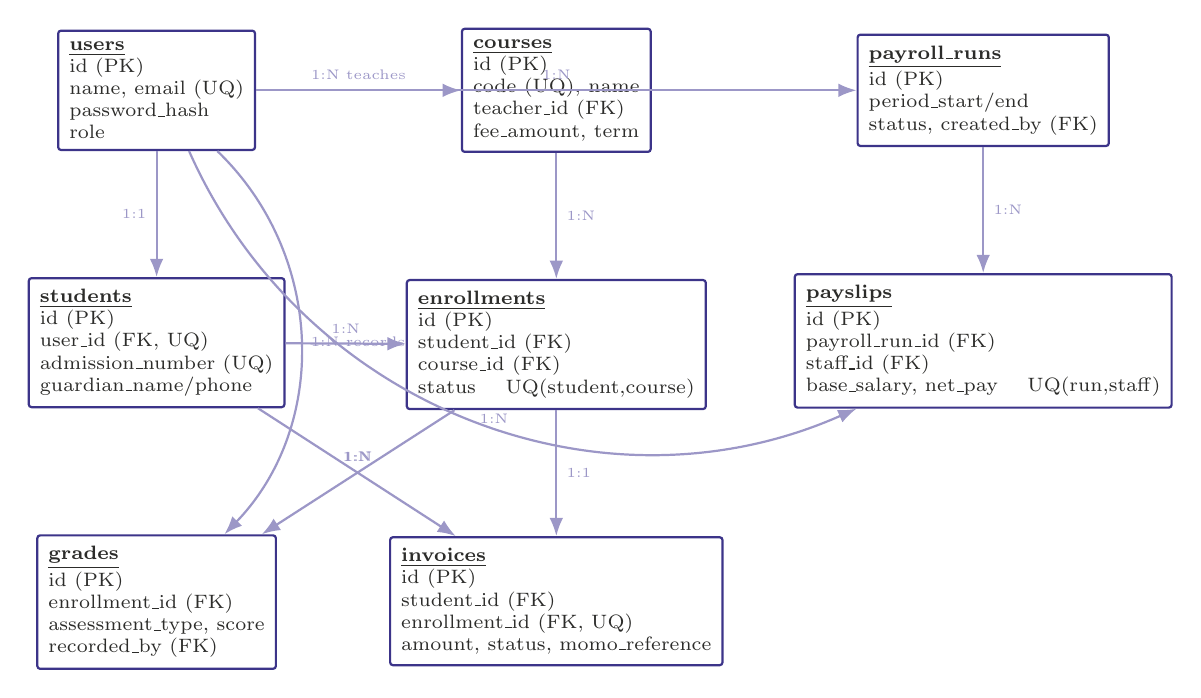
\begin{tikzpicture}[node distance=0.7cm and 1.0cm]

  \node[entity] (users) {\textbf{\underline{users}}\\ id (PK)\\ name, email (UQ)\\ password\_hash\\ role};

  \node[entity, below=1.6cm of users] (students) {\textbf{\underline{students}}\\ id (PK)\\ user\_id (FK, UQ)\\ admission\_number (UQ)\\ guardian\_name/phone};

  \node[entity, right=2.6cm of users] (courses) {\textbf{\underline{courses}}\\ id (PK)\\ code (UQ), name\\ teacher\_id (FK)\\ fee\_amount, term};

  \node[entity, below=1.6cm of courses] (enrollments) {\textbf{\underline{enrollments}}\\ id (PK)\\ student\_id (FK)\\ course\_id (FK)\\ status \quad UQ(student,course)};

  \node[entity, below=1.6cm of students] (grades) {\textbf{\underline{grades}}\\ id (PK)\\ enrollment\_id (FK)\\ assessment\_type, score\\ recorded\_by (FK)};

  \node[entity, below=1.6cm of enrollments] (invoices) {\textbf{\underline{invoices}}\\ id (PK)\\ student\_id (FK)\\ enrollment\_id (FK, UQ)\\ amount, status, momo\_reference};

  \node[entity, right=2.6cm of courses] (payrollruns) {\textbf{\underline{payroll\_runs}}\\ id (PK)\\ period\_start/end\\ status, created\_by (FK)};

  \node[entity, below=1.6cm of payrollruns] (payslips) {\textbf{\underline{payslips}}\\ id (PK)\\ payroll\_run\_id (FK)\\ staff\_id (FK)\\ base\_salary, net\_pay \quad UQ(run,staff)};

  \draw[rel] (users) -- node[left,font=\tiny]{1:1} (students);
  \draw[rel] (users) -- node[above,font=\tiny]{1:N teaches} (courses);
  \draw[rel] (students) -- node[above,font=\tiny]{1:N} (enrollments);
  \draw[rel] (courses) -- node[right,font=\tiny]{1:N} (enrollments);
  \draw[rel] (enrollments) -- node[above,font=\tiny]{1:N} (grades);
  \draw[rel] (users) to[bend left=45] node[right,font=\tiny]{1:N records} (grades);
  \draw[rel] (students) -- node[above,font=\tiny]{1:N} (invoices);
  \draw[rel] (enrollments) -- node[right,font=\tiny]{1:1} (invoices);
  \draw[rel] (users) -- node[above,font=\tiny]{1:N} (payrollruns);
  \draw[rel] (payrollruns) -- node[right,font=\tiny]{1:N} (payslips);
  \draw[rel] (users) to[bend right=45] node[right,font=\tiny]{1:N} (payslips);

\end{tikzpicture}}
\caption{Entity-Relationship Diagram for \sysname{} (PK = primary key, FK = foreign key, UQ = unique constraint). Payroll tables (right) are implemented in the schema but not yet exposed by a service.}
\label{fig:erd}
\end{figure}

\section{Notable Design Decisions}
\begin{itemize}[leftmargin=1.4em]
  \item \texttt{students} is a separate table, 1:1 with \texttt{users}, rather than adding academic-only columns to \texttt{users} -- keeps authentication identity (login/role) separate from domain profile data.
  \item There is no separate \texttt{teachers} table: a teacher is simply a \texttt{users} row with \texttt{role = 'teacher'}; \texttt{courses.teacher\_id} and \texttt{grades.recorded\_by} reference \texttt{users.id} directly.
  \item \texttt{invoices.amount} is deliberately a \emph{price snapshot at enrollment time}, not a live reference to \texttt{courses.fee\_amount} -- this is not a 3NF violation, since it represents a historical fact (``this enrollment was invoiced for this amount''), and a later fee change must not retroactively alter an issued invoice.
  \item \texttt{invoices.enrollment\_id} is \texttt{UNIQUE}, enforcing at the database level that an enrollment can never produce more than one invoice -- this is what makes the event consumer's duplicate-delivery handling (Section~\ref{sec:idempotency}) safe without extra application-level locking.
  \item Money columns use \texttt{DECIMAL(10,2)}, never \texttt{FLOAT}/\texttt{REAL}, to avoid floating-point rounding error on currency.
\end{itemize}

\section{Normalization (3NF)}
Every table is in Third Normal Form: every non-key column depends on the
whole primary key and nothing else. Fixed value sets (\texttt{role},
\texttt{status}, \texttt{assessment\_type}, \texttt{method}) use native
\texttt{ENUM} types rather than free text, preventing invalid values at the
schema level. Indexes are added on every foreign key expected to be
filtered on in a live query (\texttt{courses.teacher\_id},
\texttt{enrollments.student\_id}/\texttt{course\_id},
\texttt{grades.enrollment\_id}/\texttt{recorded\_by},
\texttt{invoices.student\_id}, \texttt{payslips.staff\_id}), beyond the
exam's 2-index minimum.

\section{UML Class Diagram}
Where Figure~\ref{fig:erd} above is a \emph{database-oriented} ER diagram
(tables, columns, keys), Figure~\ref{fig:class} is the corresponding
\emph{UML class diagram}: the same domain model expressed as classes with
typed attributes, key operations, enumerations, and every relationship kind
the UML metamodel distinguishes:
\begin{itemize}[leftmargin=1.4em]
  \item \textbf{Abstraction} -- \texttt{Person} is an abstract class (italicized, with an abstract operation); \texttt{Payable} is an interface realized by two unrelated classes.
  \item \textbf{Inheritance} (hollow triangle) -- \texttt{Admin}, \texttt{Teacher}, and \texttt{Student} all specialize \texttt{Person}.
  \item \textbf{Realization} (dashed hollow triangle) -- \texttt{Invoice} and \texttt{Payslip} both realize \texttt{Payable}.
  \item \textbf{Composition} (filled diamond) -- \texttt{Student *-- Enrollment}, \texttt{Enrollment *-- Grade}, \texttt{Enrollment *-- Invoice}: the part cannot outlive the whole.
  \item \textbf{Aggregation} (hollow diamond) -- \texttt{Course o-- Enrollment}, \texttt{PayrollRun o-- Payslip}: a weaker ``has-a'' where the part's lifecycle is not strictly bound to the whole.
  \item \textbf{Plain association} with multiplicities -- e.g. \texttt{Teacher -- Course}, \texttt{Admin -- PayrollRun}.
\end{itemize}
This is a \emph{logical/OOP} view; the physical schema (Figure~\ref{fig:erd}) implements the \texttt{Person} hierarchy as a single \texttt{users} table with a \texttt{role} discriminator column (single-table inheritance) rather than one table per subclass, as noted on the diagram itself.

\begin{figure}[h!]
\centering

\includegraphics[width=\linewidth]{figures/smartschool/02_class.png}
\caption{UML class diagram for \sysname{}, demonstrating abstraction, inheritance, realization, composition, and aggregation (PlantUML source: \texttt{figures/smartschool/02\_class.puml})}
\label{fig:class}
\end{figure}

% ================================================================
\chapter{Dynamic Behaviour}

\section{Sequence Diagram: Registration and Login}
Figure~\ref{fig:seq-auth} traces account creation and authentication. Every
lifeline carries an explicit \textbf{activation bar}: it is drawn active
only for the span between receiving a call and sending its reply, so nested
calls (Gateway waiting on Auth Service, Auth Service waiting on MySQL) are
visually unambiguous.

\begin{figure}[h!]
\centering
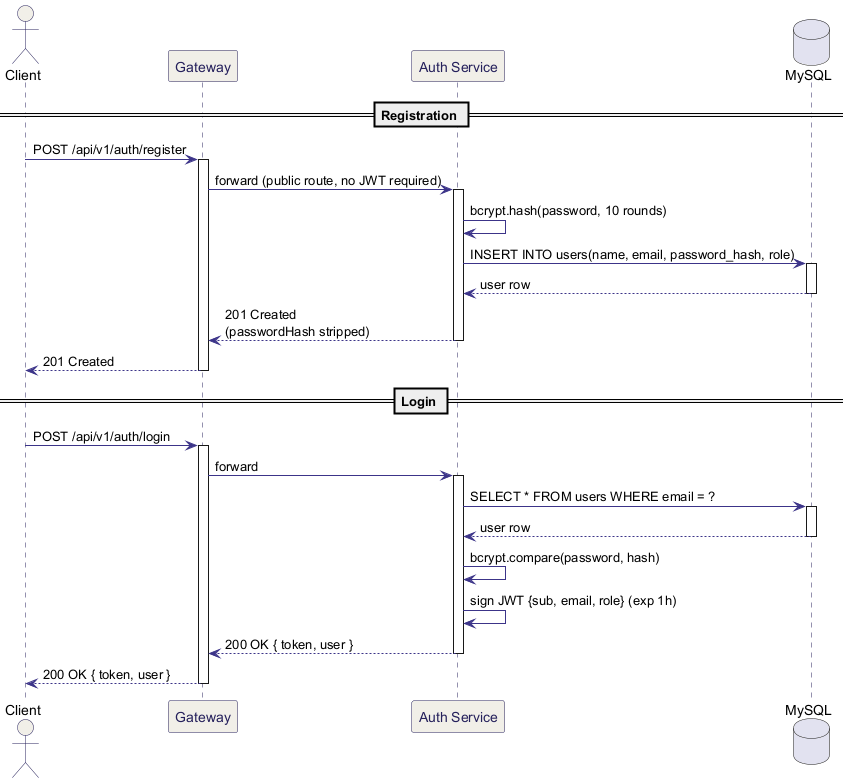
\includegraphics[width=\linewidth]{figures/smartschool/03_seq_auth.png}
\caption{Sequence diagram: registration and login, with activation bars on every lifeline (PlantUML source: \texttt{figures/smartschool/03\_seq\_auth.puml})}
\label{fig:seq-auth}
\end{figure}

\section{Sequence Diagram: Enroll in a Course (Async Invoice Creation)}
Figure~\ref{fig:seq-enroll} shows the central asynchronous workflow: the
Academic Service never waits for the Finance Service. Note where Academic
Service's activation bar ends -- \emph{before} the ``later, independently''
separator -- versus Finance Service's activation bar, which only opens once
RabbitMQ delivers the message, well after the Student already has a
response. The publish and deliver arrows use the open (async) arrowhead,
not the filled synchronous one.

\begin{figure}[h!]
\centering
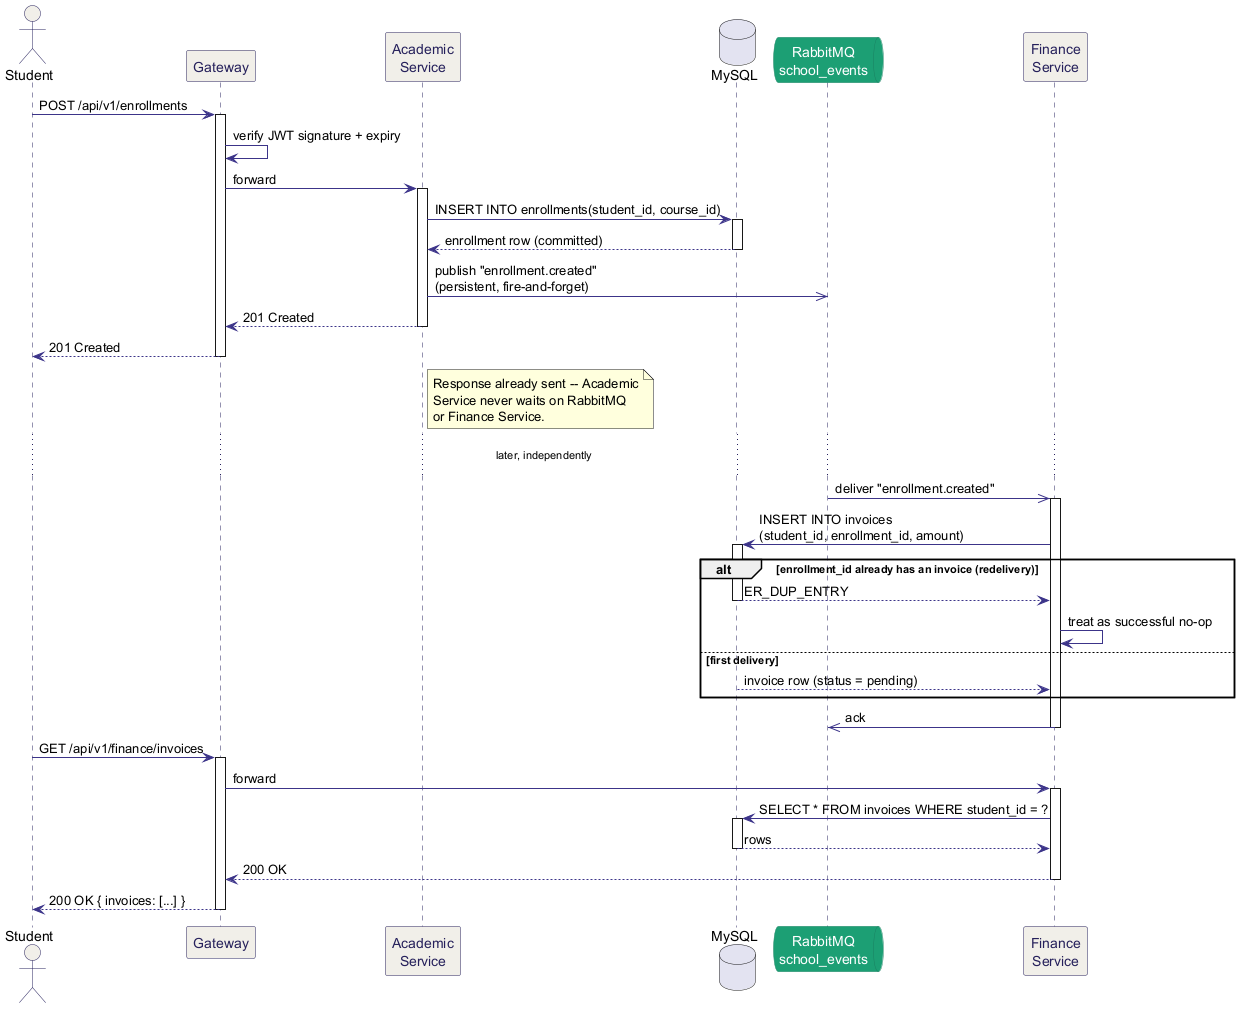
\includegraphics[width=\linewidth]{figures/smartschool/04_seq_enrollment_invoice.png}
\caption{Sequence diagram: enrollment triggers asynchronous invoice creation, with activation bars showing exactly when each participant is doing work (PlantUML source: \texttt{figures/smartschool/04\_seq\_enrollment\_invoice.puml})}
\label{fig:seq-enroll}
\end{figure}

\clearpage
\section{Sequence Diagram: Record a Grade}
Figure~\ref{fig:seq-grade} shows the ownership check that restricts a
Teacher to grading only the courses they teach, enforced independently by
Academic Service even though the Gateway already confirmed the caller is
logged in. The \texttt{alt} fragment's two branches each close their own
activation bars independently, which is standard UML for divergent
outcomes of a single call.

\begin{figure}[h!]
\centering
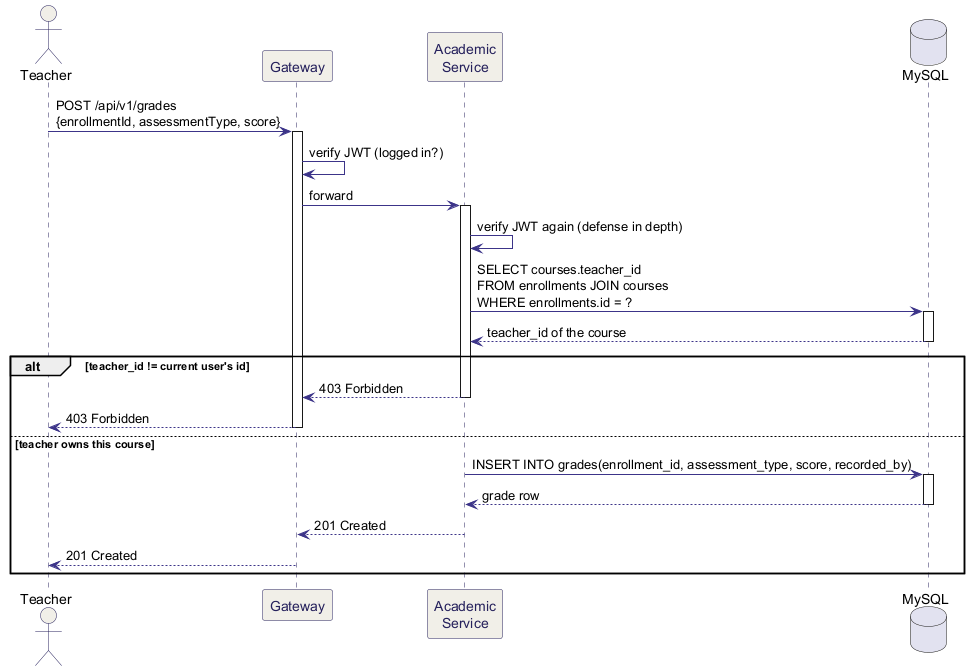
\includegraphics[width=\linewidth]{figures/smartschool/05_seq_grade.png}
\caption{Sequence diagram: recording a grade, with teacher-ownership check and full activation bars (PlantUML source: \texttt{figures/smartschool/05\_seq\_grade.puml})}
\label{fig:seq-grade}
\end{figure}

\section{State Transition Diagram: Invoice}
Figure~\ref{fig:state} shows the lifecycle of an \texttt{invoices.status}
value using full UML state-machine notation: each state has an
\texttt{entry} action, and each outgoing transition carries an explicit
\textbf{guard condition} in square brackets alongside its triggering event.
Payment collection (the \texttt{pending} $\rightarrow$ \texttt{paid}
transition, guarded on \texttt{[gateway integrated]}) is planned; today an
invoice can be created and, if applicable, cancelled, but there is no
endpoint yet that performs the \texttt{paid} transition.

\begin{figure}[h!]
\centering
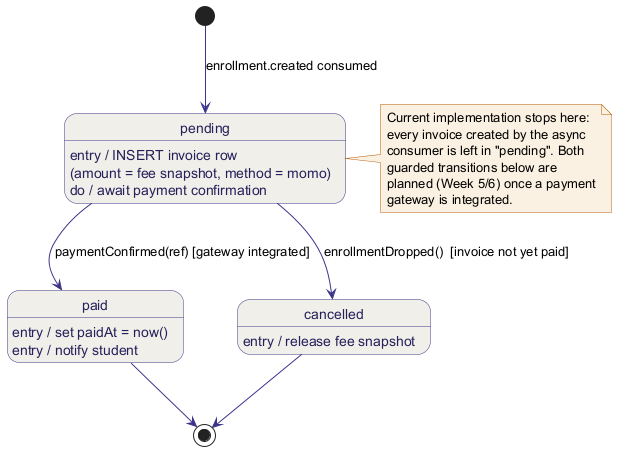
\includegraphics[width=0.7\linewidth]{figures/smartschool/07_state_invoice.png}
\caption{State transition diagram: invoice status lifecycle, with entry actions and guard conditions on every transition (PlantUML source: \texttt{figures/smartschool/07\_state\_invoice.puml})}
\label{fig:state}
\end{figure}

\section{Activity Diagram: Enrollment-to-Invoice Workflow}
Figure~\ref{fig:activity} lays out the same enrollment workflow as
Figure~\ref{fig:seq-enroll}, but as control flow rather than
inter-participant messaging, organized into \textbf{swimlanes} -- one per
participant (Student, Academic Service, RabbitMQ, Finance Service) -- so
each action's owner is unambiguous at a glance. The fork explicitly
rejoins at a single synchronization bar before the shared activity-final
node, rather than each branch terminating on its own.

\begin{figure}[h!]
\centering
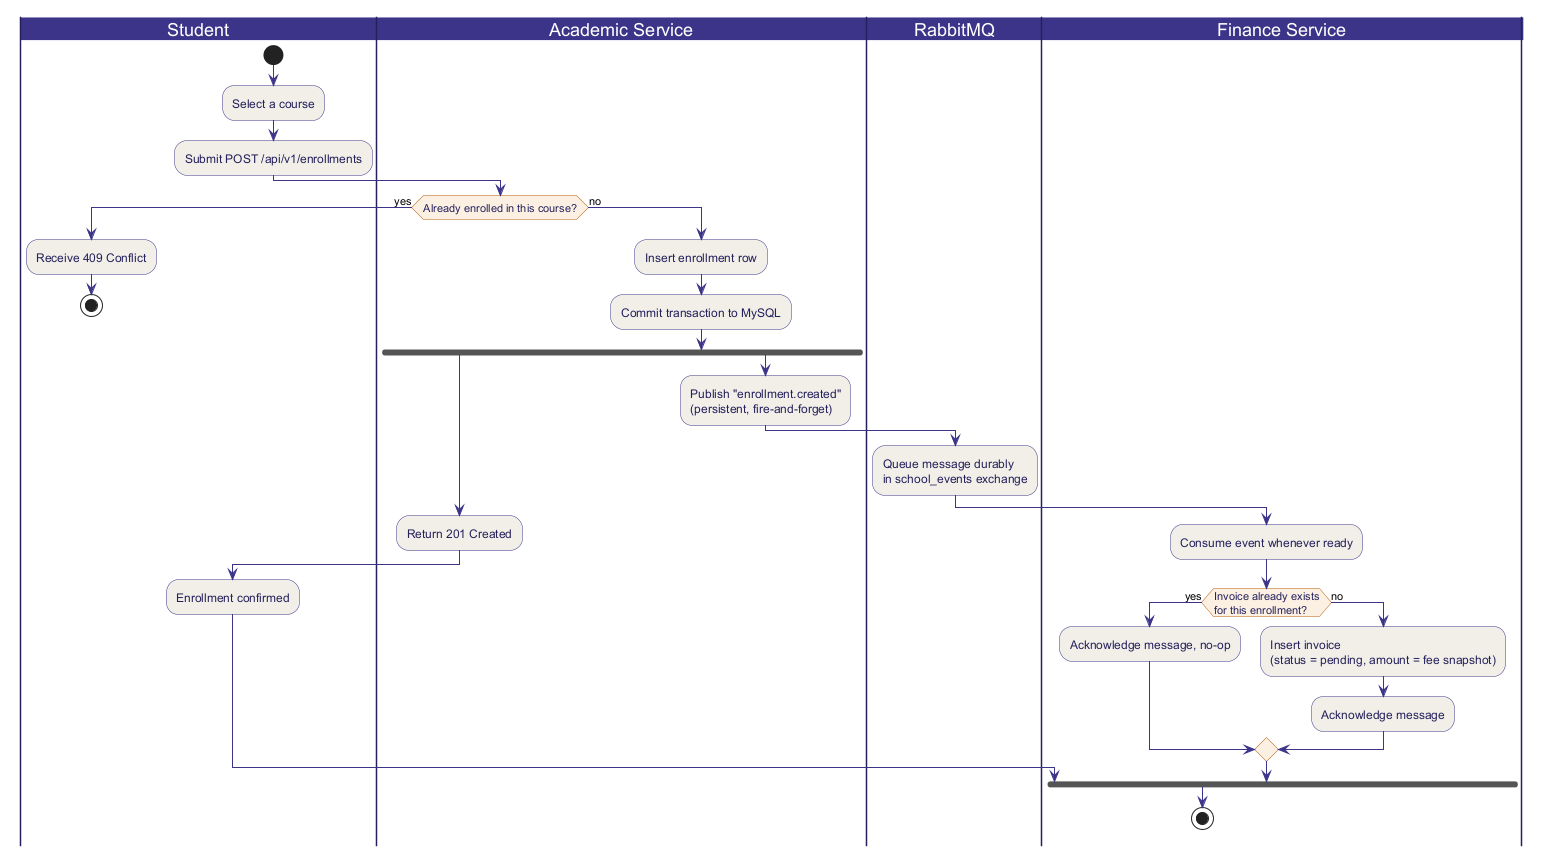
\includegraphics[width=\linewidth]{figures/smartschool/06_activity_enrollment.png}
\caption{Activity diagram: enrollment-to-invoice workflow with swimlanes, a fork into an immediate HTTP response and an independent asynchronous branch, and a single join before the final node (PlantUML source: \texttt{figures/smartschool/06\_activity\_enrollment.puml})}
\label{fig:activity}
\end{figure}

\section{Object Diagram: Sample Enrollment Snapshot}
Figure~\ref{fig:object} is a concrete runtime snapshot -- specific
instances of \texttt{Student}, \texttt{Teacher}, \texttt{Course},
\texttt{Enrollment}, \texttt{Grade}, and \texttt{Invoice}, with real
attribute values -- as a worked instantiation of the class diagram in
Figure~\ref{fig:class}. Every link is labelled with the same role name as
the corresponding class-diagram relationship (\emph{owns}, \emph{has
roster}, \emph{contains}, \emph{generates}, \emph{teaches}, \emph{records}),
so the object diagram can be read as direct proof that the class diagram's
composition and aggregation relationships hold for real data. It reuses the
same example as the event contract in Chapter~\ref{chap:api-design}, so the
two can be read side by side.

\begin{figure}[h!]
\centering
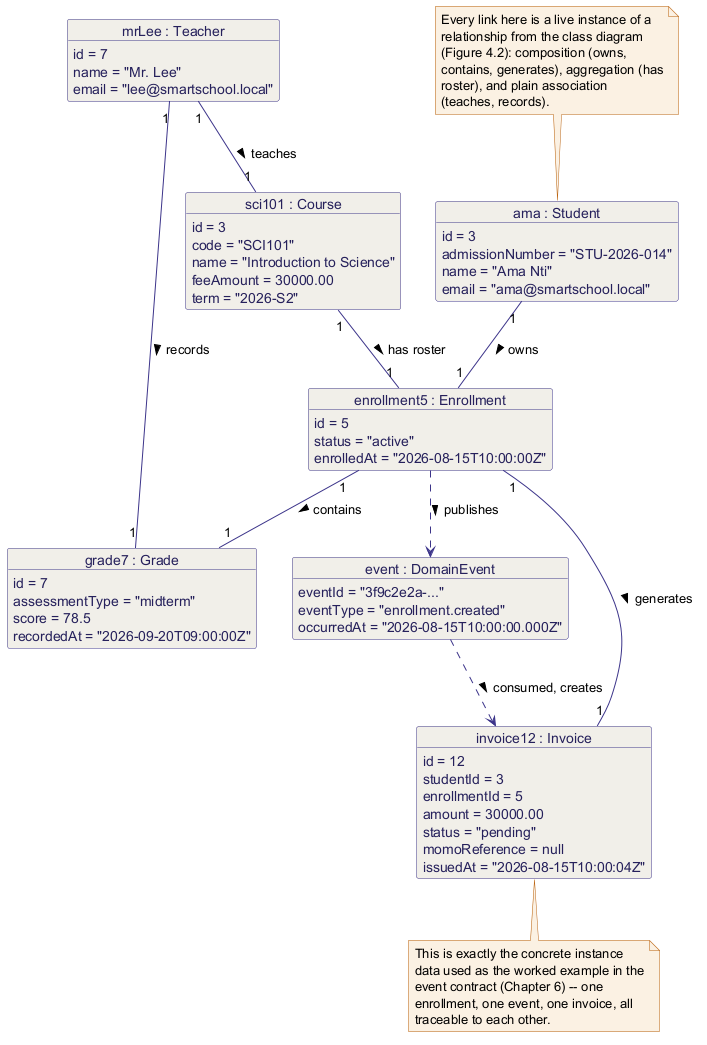
\includegraphics[width=0.8\linewidth]{figures/smartschool/08_object_snapshot.png}
\caption{Object diagram: one enrollment, its triggering event, and the resulting invoice, with links naming the same roles as the class diagram (PlantUML source: \texttt{figures/smartschool/08\_object\_snapshot.puml})}
\label{fig:object}
\end{figure}

\section{Idempotent Event Consumption}
\label{sec:idempotency}
RabbitMQ guarantees \emph{at-least-once} delivery, meaning the same
\texttt{enrollment.created} message can, in principle, be delivered more
than once (e.g. after a consumer restart before an ack is sent). The
Finance Service handles this by attempting the invoice insert and treating
a unique-constraint violation on \texttt{invoices.enrollment\_id} as a
successful no-op rather than an error -- the second delivery is
acknowledged and discarded, and the invariant ``one invoice per
enrollment'' never breaks. This is the deliberate mechanism, not an
accident: idempotency is pushed down to a database constraint rather than
implemented as fragile application-level deduplication logic.

% ================================================================
\chapter{API Design}
\label{chap:api-design}

\section{Routing Table (Gateway)}
\begin{longtable}{L{5.0cm} L{6.0cm} p{2.4cm}}
\toprule
\textbf{External path} & \textbf{Forwarded to} & \textbf{Auth} \\
\midrule
\endhead
\texttt{POST /api/v1/auth/register} & auth-service \texttt{/api/auth/register} & None \\
\texttt{POST /api/v1/auth/login} & auth-service \texttt{/api/auth/login} & None \\
\texttt{GET /api/v1/auth/me} & auth-service \texttt{/api/auth/me} & JWT \\
\texttt{GET /api/v1/reports} & auth-service \texttt{/api/reports} & JWT (admin/teacher) \\
\texttt{GET, POST /api/v1/courses} & academic-service \texttt{/api/courses} & JWT (POST: admin) \\
\texttt{GET, POST /api/v1/enrollments} & academic-service \texttt{/api/enrollments} & JWT (POST: admin/student) \\
\texttt{GET, POST /api/v1/grades} & academic-service \texttt{/api/grades} & JWT (POST: admin/teacher) \\
\texttt{GET /api/v1/finance/invoices} & finance-service \texttt{/api/invoices} & JWT \\
\bottomrule
\end{longtable}

\section{Event Contract: \texttt{enrollment.created}}
Published to the direct exchange \texttt{school\_events} with routing key
\texttt{enrollment.created}, persistent, and consumed by the
\texttt{invoice\_creation\_queue}. Figure~\ref{fig:object} in Chapter~5
renders this exact payload as an object diagram alongside the
\texttt{Student}, \texttt{Course}, \texttt{Enrollment}, and \texttt{Invoice}
instances it connects.

\begin{verbatim}
{
  "eventId": "3f9c2e2a-...",
  "eventType": "enrollment.created",
  "occurredAt": "2026-08-15T10:00:00.000Z",
  "data": {
    "enrollmentId": 5,
    "studentId": 3,
    "studentName": "Ama Nti",
    "studentEmail": "ama@smartschool.local",
    "courseId": 3,
    "courseCode": "SCI101",
    "courseName": "Introduction to Science",
    "feeAmount": "30000.00",
    "term": "2026-S2"
  }
}
\end{verbatim}

\begin{infobox}
\textbf{Why \texttt{studentId} is \texttt{students.id}, not \texttt{users.id}.}
The event carries the domain-level student id directly, so Finance Service
can insert straight into \texttt{invoices.student\_id} with no extra lookup
back to Academic Service -- keeping the two services decoupled even at the
data-access level.
\end{infobox}

% ================================================================
\chapter{Security Design}

\section{Authentication and Session Model}
Passwords are hashed with bcrypt (10 salt rounds) before storage; the raw
password is never stored or logged. On successful login, the Auth Service
issues a JWT (1-hour expiry) signed with a secret shared, via environment
variable, across every service and the Gateway. This makes sessions
stateless: any service can verify a token's authenticity without a network
call back to Auth Service.

\section{Defense in Depth}
Two independent layers check every protected request:
\begin{enumerate}[leftmargin=1.4em]
  \item \textbf{Gateway layer} -- verifies the JWT's signature and expiry before proxying at all. An invalid/missing token is rejected with \texttt{401} and never reaches a backend service.
  \item \textbf{Service layer} -- the owning service (Auth, Academic, or Finance) re-verifies the JWT and additionally enforces role/ownership rules specific to its own resources (e.g. a Teacher may only grade courses they teach).
\end{enumerate}
This split is deliberate: the Gateway is generic infrastructure answering
``is this a logged-in user at all''; business-specific authorization rules
stay with the service that owns the data.

\section{OWASP Top 10 Mitigations}
\begin{longtable}{L{3.4cm} L{10.6cm}}
\toprule
\textbf{Risk} & \textbf{Mitigation} \\
\midrule
\endhead
Injection & Every query in every service uses \texttt{mysql2} parameterized statements (\texttt{pool.query(sql, [params])}); no request value is ever concatenated into a SQL string. \\
Broken Authentication & bcrypt password hashing, 1-hour JWT expiry, and the Gateway rate limiter (10 req/60s/IP) doubling as brute-force login throttling on \texttt{/api/v1/auth/login}. Accepted gap: password policy is length $\geq 8$ only, no complexity rule -- a deliberate scope limit for a course project. \\
Sensitive Data Exposure & \texttt{password\_hash} is destructured out of every user object before it is returned (\texttt{toPublicUser()}), used by both \texttt{/register} and \texttt{/login}. Accepted gap: CORS is currently open on every service; judged low-severity since this is a Bearer-token API with no ambient cookie credential a cross-origin page could silently attach. \\
\bottomrule
\end{longtable}

% ================================================================
\chapter{Performance and Reliability}

\section{Rate Limiting}
The Gateway applies \texttt{express-rate-limit} to every route except
\texttt{/health}: 10 requests per 60 seconds per IP by default, both
externally configurable (\texttt{RATE\_LIMIT\_MAX},
\texttt{RATE\_LIMIT\_WINDOW\_MS}) without a code change. The 11th request in
a window receives \texttt{429} with standard \texttt{RateLimit-*} headers
showing remaining quota.

\section{Load Testing}
A k6 script (\texttt{load-testing/k6/gateway-load-test.js}) ramps to 20
virtual users against the Gateway. Two profiles are used:
\begin{itemize}[leftmargin=1.4em]
  \item \textbf{Safety profile} (default limits) -- proves the rate limiter engages under realistic concurrent load; the \texttt{rate\_limited\_responses} counter is non-zero.
  \item \textbf{Speed profile} (\texttt{RATE\_LIMIT\_MAX=100000}) -- measures genuine backend latency once the limiter is not a factor; the script's threshold requires \texttt{p(95) < 500ms}.
\end{itemize}

\section{Fault Tolerance in the Async Workflow}
Both the publisher (Academic Service) and the consumer (Finance Service)
connect to RabbitMQ with retry-and-backoff on startup, since a healthy
container does not guarantee AMQP is immediately ready. Publishing is
wrapped so that a RabbitMQ outage never fails or delays the enrollment HTTP
response (Section~5.2); the message, once published, is durable and
survives a broker restart. If Finance Service is stopped entirely, an
enrollment still returns \texttt{201} immediately -- the message queues up
and is drained once the service restarts, with no resend needed from
Academic Service.

% ================================================================
\chapter{Deployment View}

\section{Container Topology}
\begin{longtable}{L{2.8cm} L{4.4cm} L{4.0cm} L{2.4cm}}
\toprule
\textbf{Container} & \textbf{Published port} & \textbf{Internal address} & \textbf{Depends on} \\
\midrule
\endhead
db (MySQL 8) & \texttt{3307 $\to$ 3306} (host-only, avoids clashing with a local install) & \texttt{db:3306} & -- \\
rabbitmq & \texttt{5673 $\to$ 5672}, \texttt{15672} (mgmt UI) & \texttt{rabbitmq:5672} & -- \\
auth-service & not published & \texttt{auth-service:3000} & db \\
academic-service & not published & \texttt{academic-service:4000} & db, rabbitmq \\
finance-service & not published & \texttt{finance-service:4001} & db, rabbitmq \\
gateway & \texttt{8081 $\to$ 8080} (only published service) & \texttt{gateway:8080} & auth, academic, finance \\
\bottomrule
\end{longtable}

The whole backend starts from the repository root with a single command,
\texttt{docker compose up --build}; the frontend is a separate repository
with its own \texttt{docker-compose.yml}, started the same way, and talks
to the Gateway at \texttt{http://localhost:8081} directly from the browser.

% ================================================================
\chapter{Planned Work (Weeks 5--6)}

\begin{futurebox}
\textbf{Not yet implemented, tracked here rather than silently absent.}
\end{futurebox}

\begin{itemize}[leftmargin=1.4em]
  \item \textbf{Module feature (Week 5)} -- one complete end-to-end feature for the group's assigned module: leading candidates are payroll computation (HR: \texttt{payroll\_runs}/\texttt{payslips} already modeled) or invoice payment/reconciliation (Finance).
  \item \textbf{Automated testing and CI/CD (Week 5)} -- a first batch of automated tests for the chosen feature, and a GitHub Actions pipeline that runs them on every push.
  \item \textbf{Full integration \& documentation (Week 6)} -- a single \texttt{docker-compose} command bringing up every service, the database, the Gateway, and the message broker together (already true for the backend today; needs re-verification on a clean machine), plus the completed UML diagram set (this SDD) and this SRS kept in sync with the final system.
\end{itemize}

\end{document}
